\section{VoiceFilter}
VoiceFilter \cite{wang2019voicefilter} aims to solve the issue of The Cocktail Party Problem, where there are multiple talkers speaking simultaneously, and you want only to listen to one person, which is relatively easy to do as a human being but hard to do as a machine. The main idea of this model is to separate the Target voice using spectrogram masking.

\subsection{Model Architecture}
\begin{figure}
    \centering
    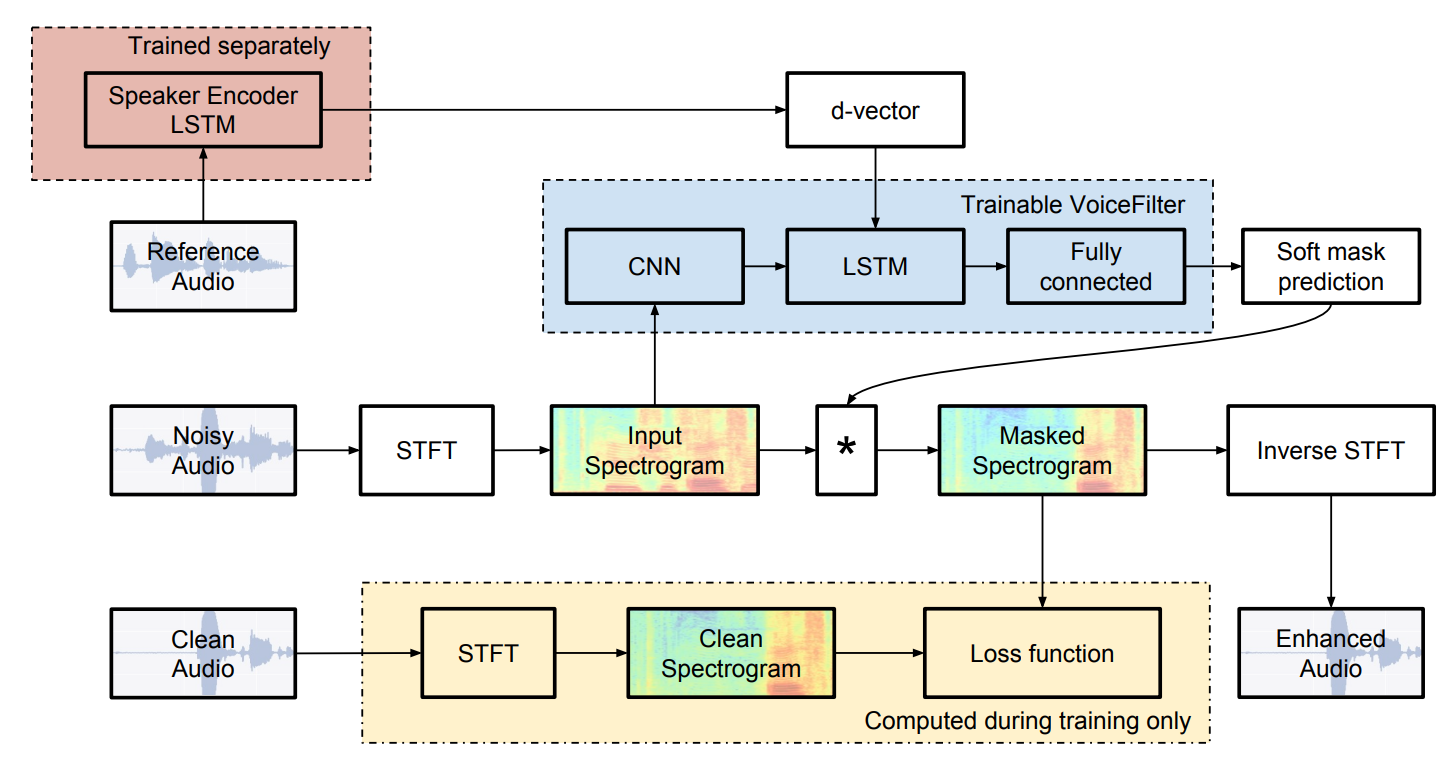
\includegraphics[width=\textwidth]{images/related_work/voicefilter/system-arch.png}
    \caption{VoiceFilter architecture}
    \label{fig:voicefilter-architecture}
\end{figure}

The architecture has two models built in which are found in Figure \ref{fig:voicefilter-architecture}:

1. Speaker Encoder (Red):
   \begin{itemize}
      \item[a.] Input: An Utterance (a sound of the speaker we target)
      \item[b.] Output: Speaker-discriminative embedding
   \end{itemize}

2. VoiceFilter (Blue):
   \begin{itemize}
      \item[a.] Inputs:
         \begin{enumerate}
            \item[i.] Magnitude Spectrogram
            \item[ii.] Speaker-discriminative embedding
         \end{enumerate}
      \item[b.] Output: Mask
   \end{itemize}


\subsubsection{Speaker Encoder}
The target speaker's audio sample is fed into the speaker encoder, which creates a speaker embedding. This system is based on recent work by Wan et al. \cite{wan2020generalized}. That delivers excellent results on speech-to-speech translation, multispeaker TTS, speaker diarization, and both text-dependent and text-independent speaker verification tasks.

A 3-layer LSTM network trained with the generalized end-to-end loss serves as the speaker encoder. It accepts log-mel filterbank energies that are taken out of 1600 ms windows as inputs and outputs 256-dimensional speaker embeddings known as $d$-vectors. We use sliding windows with $50\%$ overlap and average the $L_2$-normalized $d$-vectors that are produced on each window in order to compute a $d$-vector on a single utterance.

\subsubsection{VoiceFilter}
The recent work of Wilson et al. \cite{wilson2018}, created for voice augmentation, serves as the primary foundation for the VoiceFilter System. The target speaker's $d$-vector and a magnitude spectrogram that was calculated from a noisy audio file are the two inputs that the neural network receives. An improved magnitude spectrogram is created by multiplying the soft mask that the network predicts element-wise by the input (noisy) magnitude spectrogram. We immediately blend the noisy audio's phase with the improved magnitude spectrogram to create the enhanced waveform, and then we run an inverse STFT on the output. The goal of the network's training is to reduce the variation between the target magnitude spectrogram, which is calculated using the clean audio, and the masked magnitude spectrogram. Except the final layer, which has a sigmoid activation, the VoiceFilter network is made up of eight convolutional layers, one LSTM layer, and two fully connected layers. All of these levels have ReLU activations. Table \ref{tab:voicefilter-params} presents the values of the parameters. In each time frame, the $d$-vector is concatenated to the output of the final convolutional layer many times. The subsequent LSTM layers receive the concatenated vector as their input. For two reasons, we choose to inject the $d$-vector between the LSTM layer and the convolutional layers rather than before them. Firstly, we don't need to alter the $d$-vector by adding convolutional layers on top of it because it is already a compact and reliable representation of the target speaker. Second, convolutional layers cannot be applied to an input consisting of a magnitude spectrogram and a speaker embedding because they require time and frequency homogeneity. The input audios are split into 3-second parts for training the VoiceFilter system. If needed, they are then transformed to $16$ kHz single channel audios.

\begin{table}[htbp]
    \centering
    \begin{tabular}{|c|c|c|c|c|c|}
        \hline
        \multirow{2}{*}{\textbf{Layer}} & \multicolumn{2}{c|}{\textbf{Width}} & \multicolumn{2}{c|}{\textbf{Dilation}} & \multirow{2}{*}{\textbf{Filters / Nodes}} \\
        \cline{2-3} \cline{4-5}
        & time & freq & time & freq & \\
        \hline
        CNN 1 & 1 & 1 & 7 & 1 & 64 \\
        CNN 2 & 7 & 1 & 1 & 1 & 64 \\
        CNN 3 & 5 & 5 & 1 & 1 & 64 \\
        CNN 4 & 5 & 5 & 2 & 1 & 64 \\
        CNN 5 & 5 & 5 & 4 & 1 & 64 \\
        CNN 6 & 5 & 5 & 8 & 1 & 64 \\
        CNN 7 & 5 & 5 & 16 & 1 & 64 \\
        CNN 8 & 1 & 1 & 1 & 1 & 8 \\
        LSTM  & - & - & - & - & 400 \\
        FC 1  & - & - & - & - & 600 \\
        FC 2  & - & - & - & - & 600 \\
        \hline
    \end{tabular}
    \caption{Parameters of the VoiceFilter network.}
    \label{tab:voicefilter-params}
\end{table}

\subsection{Experimental Setup}

\subsubsection{Dataset}
Using two datasets concatenated, the MultiReader approach described in \cite{wan2020generalized} was used to train the Speaker Encoder. Anonymized voice query records in English from mobile and far-field devices make up the first dataset. The dataset that comprises LibriSpeech \cite{librispeech}, VoxCeleb, and VoxCeleb2 is the second one. Additionally, VoiceFilter was trained using data that was generated by the original authors and came from either the LibriSpeech or the VCTK dataset. Ten speakers were used for testing and 99 speakers for training in VCTK. They used the training and development sets—2338 speakers in the training set and 73 speakers in the development set—that were specified in the dataset's procedure for LibriSpeech. Each utterance in these two read speech datasets features the voice of a single speaker.
And the data generation flow is shown in Figure \ref{fig:voicefilter-data}.

\begin{figure}
    \centering
    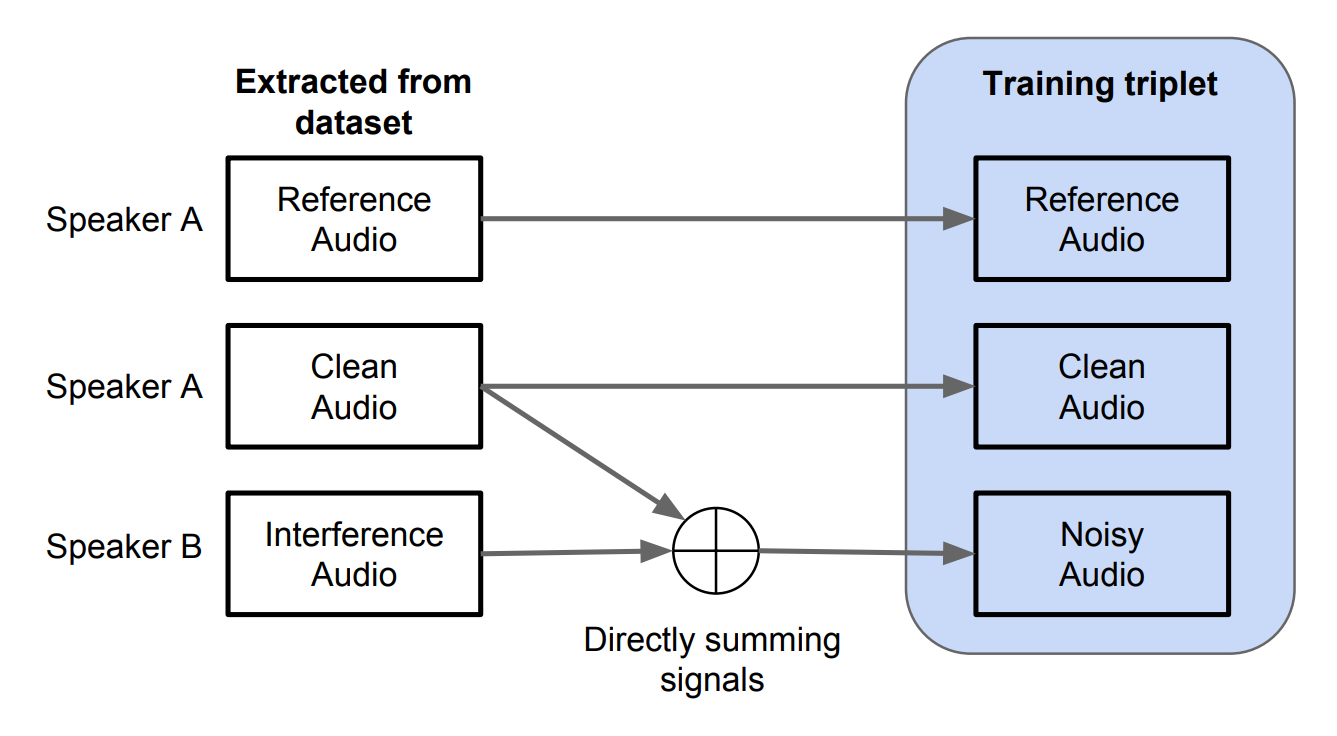
\includegraphics[width=0.8\textwidth]{images/related_work/voicefilter/data-proc.png}
    \caption{Input data processing workflow.}
    \label{fig:voicefilter-data}
\end{figure}

\subsubsection{Evaluation}
To evaluate the performance of different VoiceFilter models, we use two metrics: the speech recognition Word Error Rate (WER) and the Source to Distortion Ratio (SDR).

\paragraph{Word Error Rate (WER)}\mbox{}\\
Four WER numbers were important to them: 
\begin{itemize}
    \item \textbf{Clean WER:} The WER on the clean audio, without VoiceFilter.
    \item \textbf{Noisy WER:} The WER on the noisy (clean + interference) audio in the absence of VoiceFilter.
    \item \textbf{Clean-enhanced WER:} The WER on the clean audio that the VoiceFilter system processed.
    \item \textbf{Noisy-enhanced WER:} The WER on the loud audio that the VoiceFilter system processed.
\end{itemize}
These two characteristics should be present in a decent VoiceFilter model: 
\begin{itemize}
    \item Since noisy-enhanced WER is much lower than noisy WER, the VoiceFilter is helping with multi-speaker speech recognition.
    \item Clean-enhanced WER is quite close to Clean WER, indicating that in single-speaker circumstances, the VoiceFilter has few adverse effects.
\end{itemize}

\paragraph{Source-to-Distortion Ratio (SDR)}\mbox{}\\
A popular statistic for assessing source separation systems is the SDR, which necessitates knowledge of both the augmented and clean signals. It is a dB-expressed energy ratio that compares the energy of the target signal—which is contained in the boosted signal—to the energy of the mistakes, which are caused by artifacts and interfering speakers. Therefore, the higher, the better.